\documentclass{article}
\usepackage[utf8]{inputenc}
\usepackage[spanish]{babel}
\usepackage{listings}
\usepackage{graphicx}
\graphicspath{ {images/} }
\usepackage{cite}

\begin{document}

\begin{titlepage}
    \begin{center}
        \vspace*{1cm}
            
        \Huge
        \textbf{Analisis y diseño}
            
        \vspace{0.5cm}
        \LARGE
        Parcial 2
            
        \vspace{1.5cm}
        \textbf{Miguel Angel Serna Montoya}
            
        \vfill
            
        \vspace{0.8cm}
            
        \Large
        Departamento de Ingeniería Electrónica y Telecomunicaciones\\
        Universidad de Antioquia\\
        Medellín\\
        Septiembre de 2021
            
    \end{center}
\end{titlepage}

\tableofcontents

\section{Análisis problema} \label{contenido}
1er día: Por el momento mis ideas algorítmicamente hablando son casi nulas por no decir obsoletas ya que no he podido dedicarle el merecido tiempo al planteamiento del problema. Por el momento me estoy encargando de entender bien los requisitos y restricciones con los que me veo comprometido.
2do día: Me doy cuenta viendo la repetición de la clase que el principal desafió es el de desarrollar las funciones de submuestreo o sobremuestrueo. Creare una clase llamada lecturaEscritura que va a leer los valores de la imagen y los almacene en un vector tridimensional y también tendrá un método para escribir el txt, le voy a entregar este vector tridimensional de valores a un método de la clase escalado que se encargara de sobremuestrear o submuestrear la imagen. Luego el vector tridimensional final(Con la imagen ya escalada) se lo entrego a un método de  la clase de lecturaEscritura que se encargara de escribir los datos en un txt.
\section{Consideraciones}
No puedo usar las librerías para el submuestreo o sobremestrueo. Todo tiene que ser de mi puño y letra.
No importa el tamaño de la imagen. Hoy estuve en esas todo el día.
Tengo que considerar el formato de salida para que solo sea copiar y pegarlo en el código de tinkercad.
\newpage
\section{Diseño algoritmo}
\begin{figure}[h]
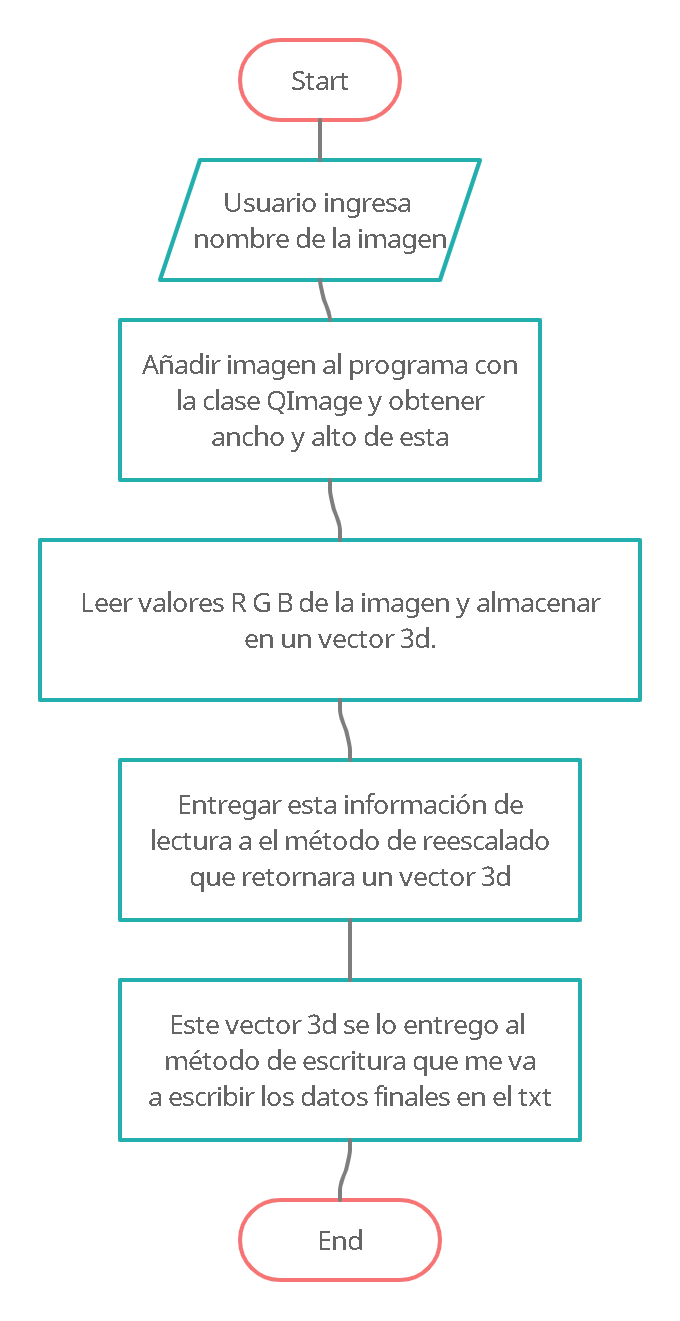
\includegraphics[width=7cm]{imag-analisis/DisenoAlgoritmo.png}
\centering
\caption{diseño}
\label{fig:diseño}
\end{figure}
\newpage
\section{Esquema de tareas}
\begin{figure}[h]
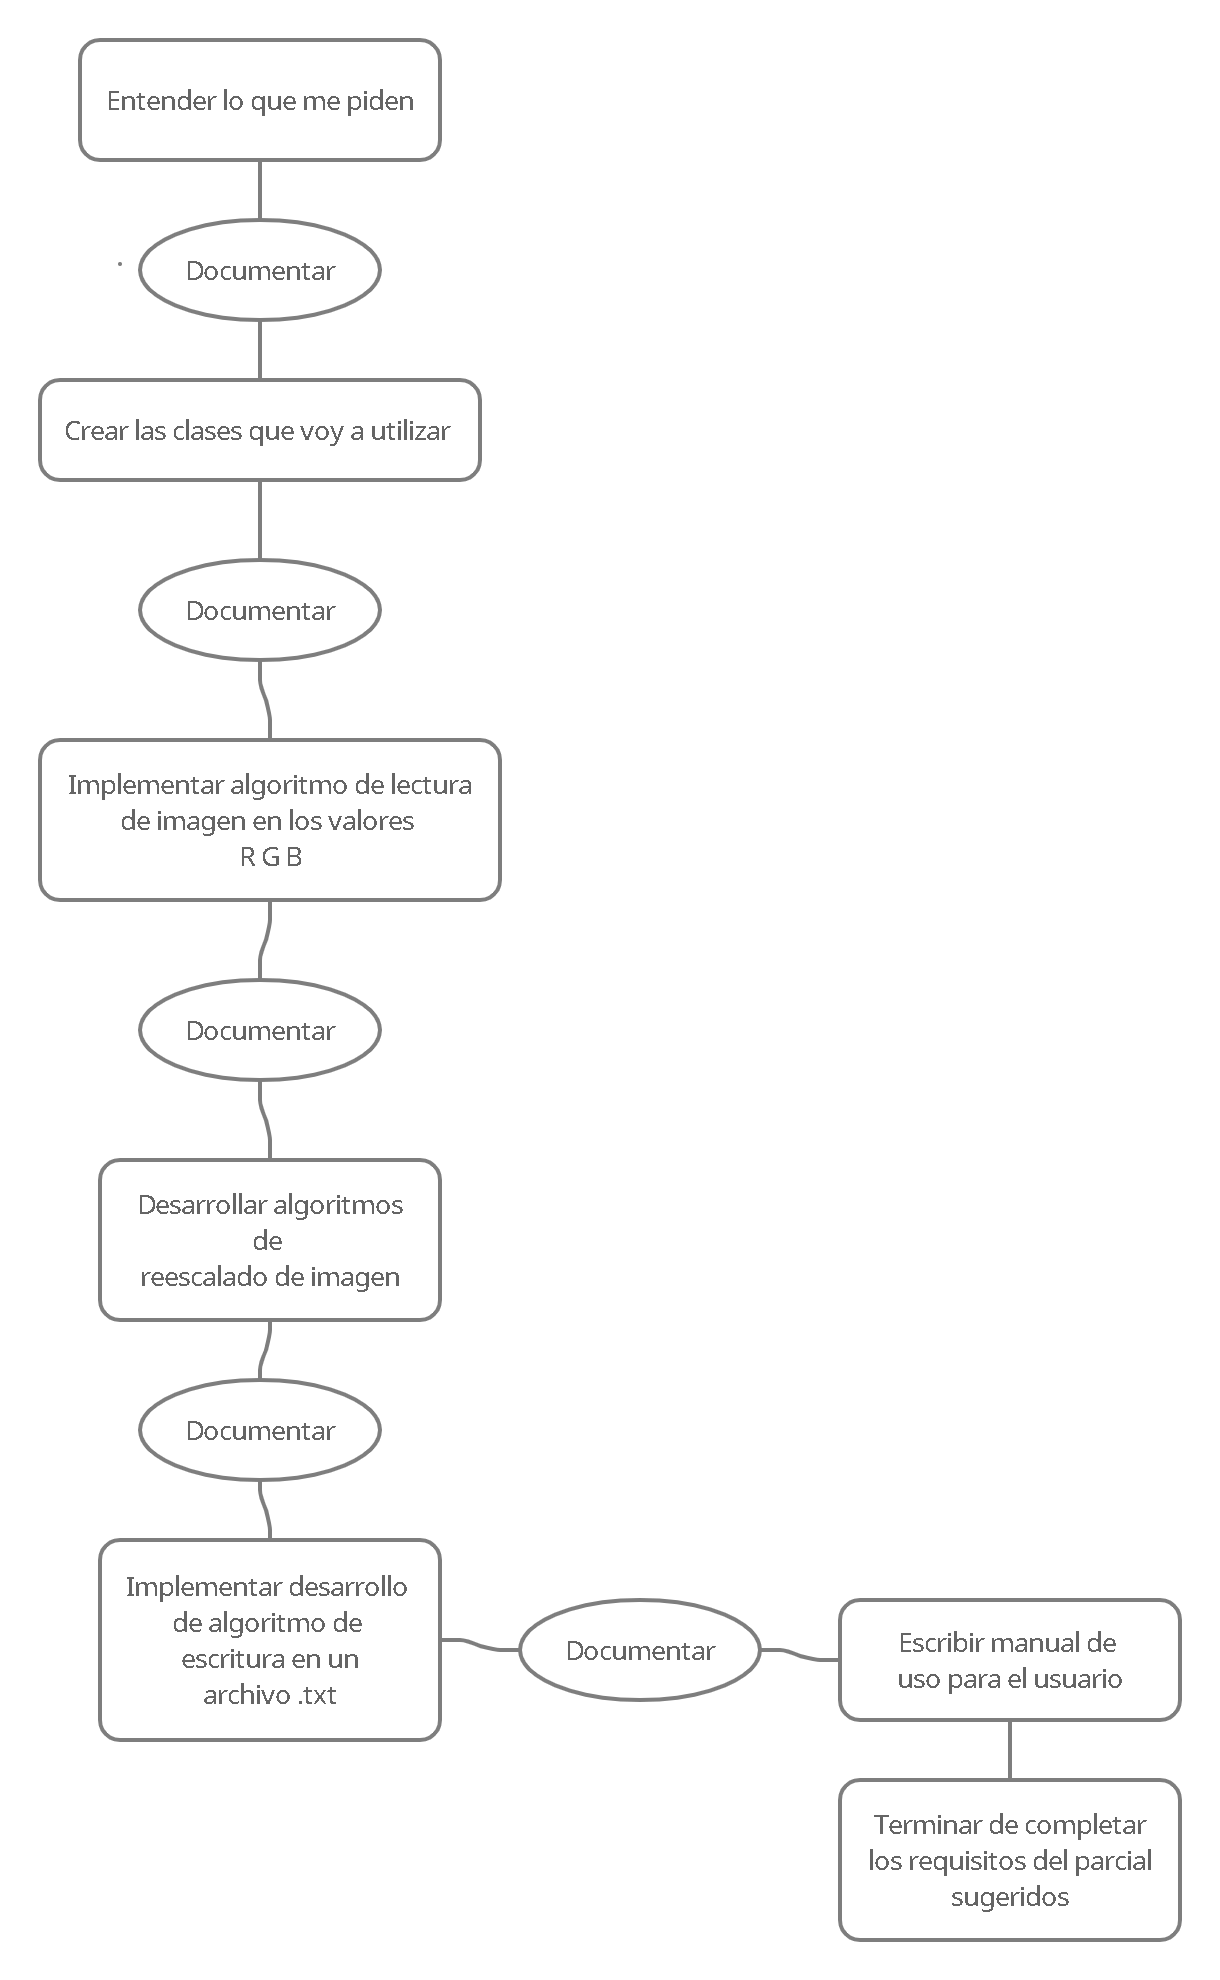
\includegraphics[width=7cm]{imag-analisis/esquema.png}
\centering
\caption{esquema}
\label{fig:esqueme}
\end{figure}


\end{document}